\section{mbeddr}


The mbeddr open-source project\footnote{ \url{http://mbeddr.com}} 
focuses on supporting embedded software
development. It introduces a set of of modular domain-specific extensions
to C and also supports other languages for addressing common problems 
in software development, \eg writing documentation with close 
integration to code or capturing requirements. mbeddr is build using 
JetBrains \ac{MPS} language 
workbench\footnote{ \url{https://www.jetbrains.com/mps/}}.
\fig{mbeddrArch} shows how mbeddr is organized into layers, with \ac{MPS} at
the bottom and custom language extensions on top.
\ac{MPS} supports the definition, 
composition and use of general purpose or domain-specific languages. 
To archive this \ac{MPS} uses a projectional editor, this means, even 
if the notation might look textual it is not represented as a sequence 
of characters, which are transformed into a \ac{AST} by parsing. 
In contrast user actions manipulate the \ac{AST} directly. The \ac{AST} 
is then rendered to the user according to editor specifications/projection
rules. These rules are not limited to textual notations, for example can tabular
or mathematical notations can be used if appropriated. Since no parsing ambiguities 
can occur a wide range of languages extension can be supported.

\begin{figure}[h]
  \vspace{-2mm}
  \centering
    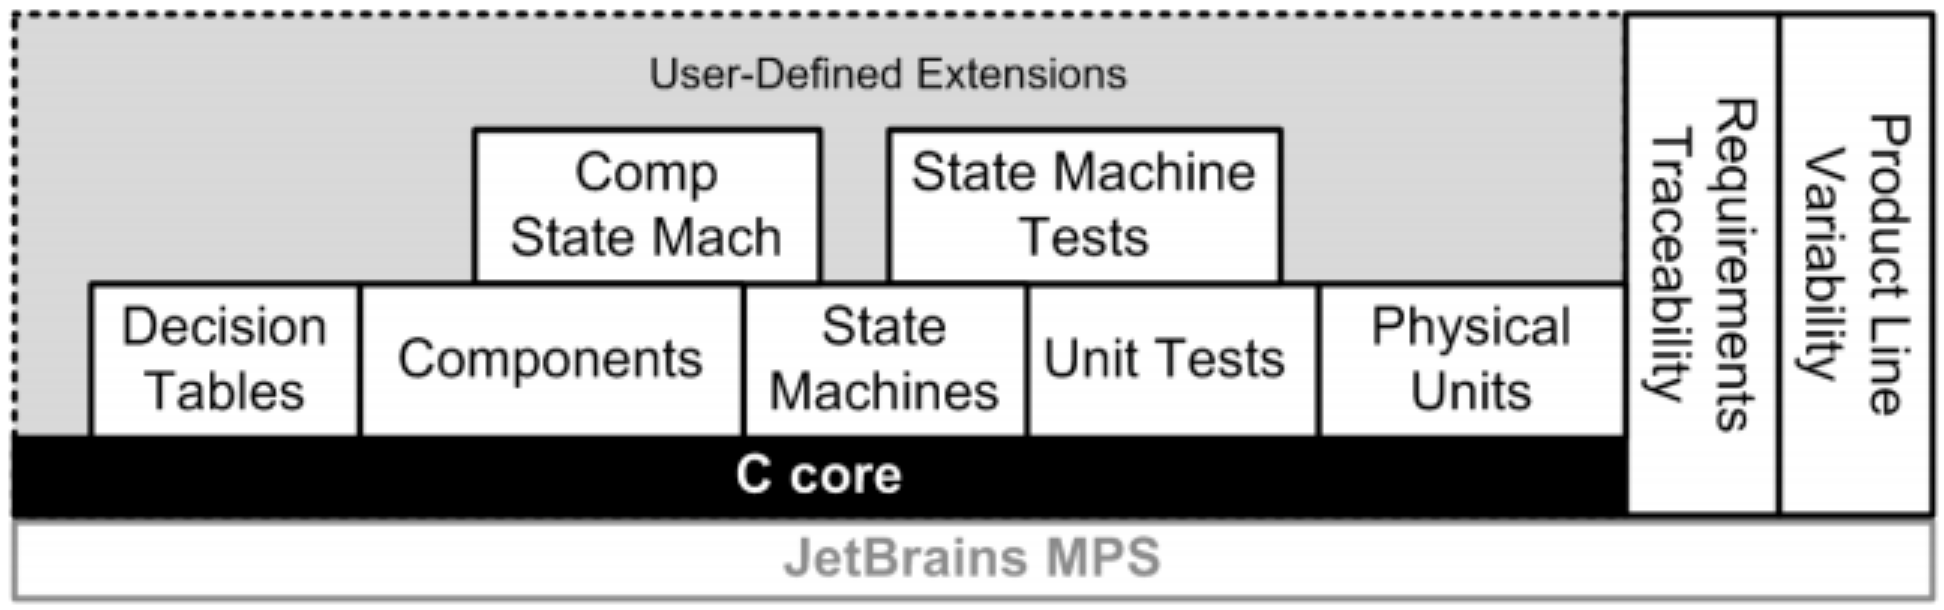
\includegraphics[width=8.5cm]{./figures/mbeddArch.png} 
    \vspace{-2mm}
    \caption{mbeddr language architecture~\cite{Voelter:2012:MEC:2384716.2384767}}
  \label{mbeddrArch}
  \vspace{-2mm}
\end{figure}


\subsection{Languages}
\label{languageImplementation}
mbeddr includes a extensible C99 implementation. In addition to plain C 
mbeddr also include a set of predefined extension on top of C. These 
extension include test cases, state machines, components and physical units. 
In \ac{MPS}, languages are separated into modular aspects. 
The major aspects 
of a language are described below. However, for building debugging support
we only care about \ic{Structure}, \ic{Generator} and constraints expressed in  
\ic{Type System/Contraints}.

\parhead{Structure:} Definition of the \ac{AST} of the language.

\parhead{Editor:} Projection rules how the \ac{AST} is presented to the user and how the user interacts with the program.

\parhead{Type System/Contraints:} Static semantics of the language.
 
\parhead{Generator:} Dynamic semantics of the language, transforms the model into executable code.

\subsection{Unit Test Language Extension}

In this section we will build a language extension
for writing test cases with mbeddr.\footnote{The language design is derivded 
from mbeddr's \ic{unittest} language.}  In the later sections we will show
how to build debugging support for this langauge and how to test its debugging
support.

\noindent \textbf{Structure:}

\fig{fig:UnitTestStructure} shows the language structure, which we discuss now
in detail. \ic{AssertStatement} is derived from \ic{Statement} and can therefore
be used where \ic{Statement}s are epected. It contains an \ic{Expression}, which
represents the \emph{condition}.
\ic{TestCase} holds a \ic{StatementList}, which contains the \ic{Statement}s
that make up the test. Further, \ic{TestCase} implements \ic{IModuleContent},
which makes the concept usable on top level of mbeddr \ic{Module}s (a
compilation unit). Other subconcepts of this marker interface are 
\ic{GlobalVariableDeclartion} or \ic{Function}.
An \ic{ExecuteTestExpression} is an \ic{Expression} and contains a list of
\ic{TestCaseRef}. Those references refer to \ic{TestCase} to be executed.

\begin{figure}[h]
  \vspace{-2mm}
  \centering
    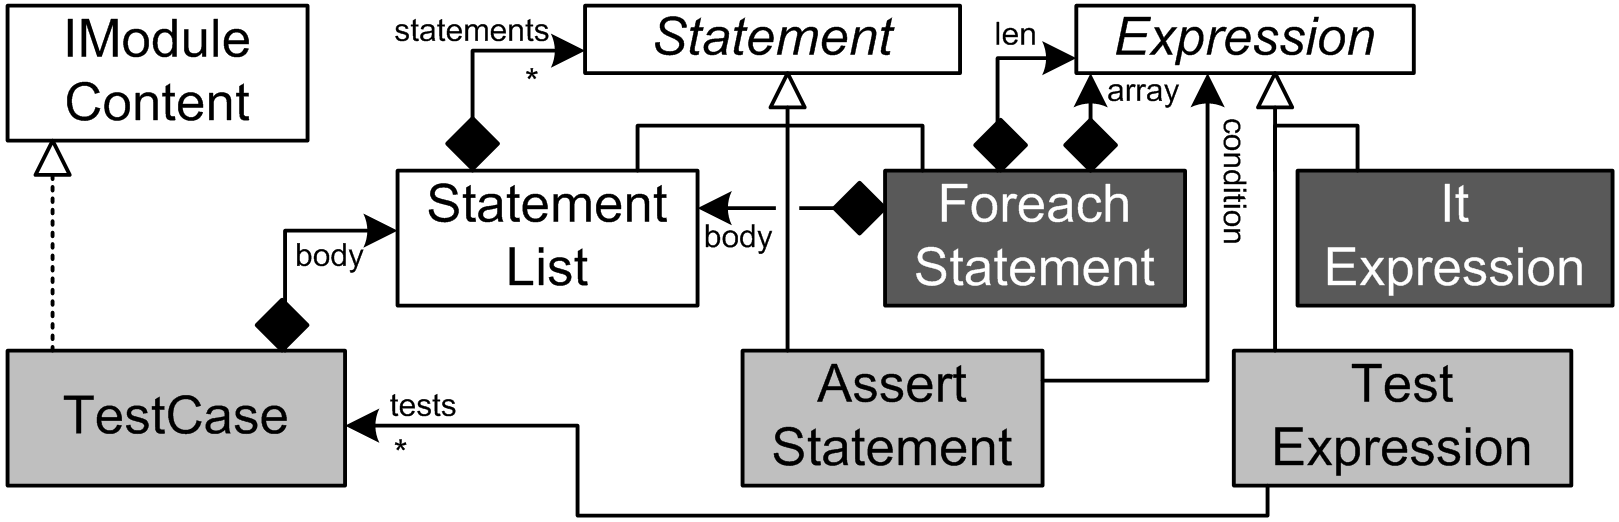
\includegraphics[width=8.5cm]{./figures/umldiag.png} 
    \vspace{-2mm}
    \caption{Language structure}
  \label{fig:UnitTestStructure}
  \vspace{-2mm}
\end{figure}

\parhead{Type System/Constraints:}

For implementing our \ic{AssertStatemnt} we require a constraint and a type
system rule. First restricts the usages only inside \ic{TestCase}s, meaning an
\ic{AssertStatemnt} must always live inside (considering the \ic{AST}) a
\ic{TestCase}:
\begin{lstlisting}[language=mbeddr,frame=single]
parentNode.ancestor<concept = TestCase, +>.isNotNull
\end{lstlisting}

Second restricts the type of its child \ic{expr} (the condition) to
\ic{BooleanType}, so only valid \emph{conditions} can be entered:
\begin{lstlisting}[language=mbeddr,frame=single]
check(typeof(assertStatement.expr) :<=: <BooleanType()>);
\end{lstlisting}

Since \ic{ExecuteTestExpression} is an expression, which returns a value (the
number of failures), we specify \ic{Int32tType} as its type (see rule below). We
will later use the same type inside the code generator.
\begin{lstlisting}[language=mbeddr,frame=single]
check(typeof(executeTestExpression) :==: <Int32tType()>);
\end{lstlisting}


\parhead{Generator:}

Our generator consists of many different transformation rules, which translate  
code written with our language directly to mbeddr C. \lst{lst:generatedUT} shows
on the left hand side an example program, written with mbeddr C and our language
extension. The right hand side shows the resulting C program. While
regular mbeddr code is not colored, the boxes show how \ac{AST} nodes from the
left are translated to C code on the right.

\noindent 
\hspace{1.2mm}
\begin{minipage}[t]{120pt} 
\begin{lstlisting}[language=reducedMbeddr,numbers=left]
int32 main(int32 argc,
		string[] argv) {
   return $\colorbox{g1}{test[}$$\colorbox{g6}{forTest}$$\colorbox{g1}{]}$;
}
$\colorbox{white}{\hspace{2mm}{\color{white}\_f;}}$
$\colorbox{white}{\hspace{2mm}{\color{white}blockexpr\_2();}}$
$\colorbox{white}{\hspace{2mm}{\color{white}\}}}$
$\colorbox{white}{\hspace{2mm}{\color{white}\}}}$
$\colorbox{white}{\hspace{2mm}{\color{white}int32\_t bp\_2() \{}}$ 
$\colorbox{white}{\hspace{2mm}{\color{white}i32\_t \_f = 0;}}$		

$\colorbox{g7}{testcase forTest \{}$ 
$\colorbox{white}{\hspace{2mm}{\color{white}|}}$
   int32 sum = 0;
$\colorbox{g3}{\hspace{2.5mm}assert:}$ sum == 0$\colorbox{g3}{;}$   
   int32[] nums = {1, 2, 3};
   for(int32_t i=0;i<3;i++){
     sum += nums[i];
   }
$\colorbox{g3}{\hspace{2.5mm}assert:}$ sum == 6$\colorbox{g3}{;}$
$\colorbox{white}{{\color{white}\_f++;}}$
$\colorbox{g7}{\}}$
\end{lstlisting}
\end{minipage} 
\rule[-53ex]{0.1ex}{24.0em}
\hspace{0.75mm}
\begin{minipage}[t]{125pt} 
\begin{lstlisting}[language=reducedMbeddr,numbers=left]
int32_t main(int32_t argc,
		char *(argv[])) {
   return $\colorbox{g1}{blockexpr\_2()}$;
}  
$\colorbox{white}{\hspace{2.5mm}{\color{white}|}}$
$\colorbox{g1}{int32\_t blockexpr\_2(void) \{}$
$\colorbox{g1}{\hspace{2.5mm}int32\_t \_f = 0;}$
$\colorbox{g6}{\hspace{2.5mm}\_f += test\_forTest();}$
$\colorbox{g1}{\hspace{2.5mm}return \_f;}$
$\colorbox{g1}{\}}$

$\colorbox{g7}{int32\_t test\_forTest() \{}$
$\colorbox{g7}{\hspace{2.8mm}int32\_t \_f = 0;}$
   int32_t sum = 0;
$\colorbox{g3}{\hspace{2.8mm}if(!(}$sum == 0$\colorbox{g3}{)) \{ \_f++; \}}$
   int32_t[] nums = {1, 2, 3};
   for(int32_t i=0;i<3;i++){
     sum += nums[i];
   }
$\colorbox{g3}{\hspace{2.8mm}if(!(}$sum == 6$\colorbox{g3}{)) \{ \_f++; \}}$
$\colorbox{g7}{\hspace{2.8mm}return \_f;}$
$\colorbox{g7}{\}}$
\end{lstlisting}
\end{minipage} 
\vspace{-1mm}
\begin{lstlisting}[caption={Example mbeddr program using the unit test language
on the left and the C code that has been generated from it on the right. Empty
lines on the left have no meaning, they are used for showing the relationship
between high-level and generated code.},language=mbeddr,label=lst:generatedUT]
\end{lstlisting}

